\section{Optimization}
\begin{enumerate}
    \item \textbf{define optimization problem} on ($\ell$, I, b, $\Delta \phi$), we leave $\Delta \theta$ and verify later that it has little impact
    \textbf{Assumption}: $\Delta \theta$ has little impact over the result

    maximize average power, BVP as constraint

instead of tf -> infty + arbitrary IC, we let tf be the period, such that tau(tf) = tau(t0) + 2pi, initial condition such that tau(t0) = 0

\item \textbf{solve and compare} with PTO init (statistics + trajectories)

\%gain, line tension, other qualitative remarks ?

\item \textbf{verify that $\Delta \theta$ has little impact} over [2°, 20°]: negligible change on power and tension

\item \textbf{Landscape of the objective around the optimum}: vary (l, I, b, $\Delta \phi$), then vary wind speed
\end{enumerate}

We designed this model to evaluate the average power output of KEEP. In section \alter{section}, we computed the average power \alter{did we? or was is only a limit cycle without power?} for a set of environment and design parameters by computing its limit cycle, now we will fix the environment, mainly the reference wind speed \(v_\mathrm{ref}\), and maximize the average power output by tuning a selection of design parameters over one revolution of a periodic orbit \alter{do we keep 'limit cycle'?}.

\alter{>>>>>>>>>>>>>>>>>> Put this in section 2 ?}
The average power is given by
\begin{equation}
    \bar P = W_f/t_f
\end{equation} where \(W_f\) is the total work done during one limit cycle and \(t_f\) is its period. We augment the state of our dynamical system with \(W\) that verifies:
\begin{equation}
\begin{cases}
    W(0) = 0 \\
    \dot W(t) = \dot W(t) = - \dot \alpha \, T(\dot \alpha) = b \, \dot \alpha^2 \quad (\geq 0),
\end{cases}
\end{equation}
\alter{<<<<<<<<<<<<<<<<<<<}
then we define the total work as:
\begin{equation}
    W_f = W(t_f).
\end{equation}
\alter{I repeat "numerical integration" this after stating the constraints of the problem}
The augmented state variable \(W\) is solved concurrently with \(\vb x\), using the same numerical scheme (Runge-Kutta), such that we define the augmented state \(\tilde{\vb x} = (\vb x, W) \) \alter{can we avoid this definition?}.

\alter{>>>>>>>>>>>>>>>>>> Put this in section 2 ?}
For the solution of the \ac{ivp} to be a periodic orbit, the additional looping constraints must be enforced:
\begin{equation}
\begin{split}
    \alpha(t_f)      &= \alpha(0) \\
    \tau(t_f)        &= \tau(0) \pm 2\pi \\
    \dot \alpha(t_f) &= \dot \alpha(0) \\
    \dot \tau(t_f)   &= \dot \tau(0),
\end{split}
\end{equation}
which yields a \ac{bvp}. \alter{define this in the "finding a limit cycle section"}
Without loss of generality, we can fix the phase by imposing
\begin{equation}
    \tau(0) = 0,
\end{equation}
 it follows that
\begin{equation}
    \tau(t_f) = \pm 2\pi
\end{equation}
where \alter{this is probably going to be a repeat of section 2} the sign determines the direction of travel of the kite: either it rises on the sides of the eight (\(\tau(t_f) = +2\pi\)) or in its center (\(\tau(t_f) = -2\pi\)). To avoid the lines sliding against each other, we choose the former
\begin{equation}
    \tau(t_f) = +2\pi.
\end{equation}
\alter{<<<<<<<<<<<<<<<<<<<}

We bundle \alter{these equations (give them labels and reference them?)} into the following optimization problem:
\begin{equation}
W_f / t_f \underset{\substack{\alpha_0, \dot{\alpha}_0, \dot{\tau}_0 \\ W_f, t_f \\ \Theta}}{\longrightarrow} \max
\end{equation}
subject to constraints
\begin{equation}\begin{split}
    &\alpha(t_f, \Theta) = \alpha_0 \\
    &\tau(t_f, \Theta) = \tau_0 + 2\pi\\
    &\dot \alpha(t_f, \Theta) = \dot \alpha_0 \\
    &\dot \tau(t_f, \Theta) = \dot \tau_0 \\
    &W(t_f, \Theta) = W_f;
\end{split}
\end{equation}
we compute the state at \(t_f\) by numerically solving the \ac{ivp} given initial condition \(\tilde x(0) = (\alpha_0, 0, \dot \alpha_0, \dot \tau_0, 0)\) and parameters \(\Theta\), using an adaptive Runge-Kutta scheme \addcite{.}. The optimization problem itself is solved using the interior point method implemented in Ipopt \addcite{.} with linear solver Mumps \addcite{.}, while ForwardDiff.jl \addcite{.} efficiently \alter{automatically, algorithmically?} evaluates all required derivatives.

\alter{- intial guess}

We start with physically-reasonable values for the parameters \(\Theta\) \alter{can we get them from Alain's model? That would be very cool! "We start with values obtained from  annex X where we use a kinematic model to determine the optimal parameters..."}, compute the corresponding limit cycle, from which we \alter{infer, extract, obtain} the initial guess for \(\alpha_0, \dot \alpha_0, \dot \tau_0, t_f\), and \(W_f\); this process results in an \alter{a pre-optimized} feasible point.



\alter{- implementations, used packages}




where \(W\)
Given a vector of parameter values \alter{set of parameters -- more less mathy but better?}, we evaluate the average power by integrating the instantaneous power using the same Runge-Kutta method we use for solving the \ac{ivp}, resulting in a new -- augmented -- state, \(W\), for \emph{work}:
\begin{equation}
    \begin{cases}
        W(0) = 0
        \dot W(t) = - \dot \alpha \, T(\dot \alpha) = b \, \dot \alpha^2 \quad (\geq 0),
    \end{cases},
\end{equation}
where the instantaneous power \(\dot W\) is the product between (the opposite of) the torque and the arm angular velocity.
The \emph{average} power is then the ratio between the final work \(W(t_f)\) over the period of the limit cycle \(t_f\).
For a given \alter{set of parameters}, we will determine:
\begin{itemize}
    \item \(\alpha_0, \dot \alpha_0, \dot \tau_0\)
\end{itemize}

: arm inertia \(I\), linear torque \(b\) coefficient and line length \(\ell\). We denote by \(\Theta = (I, b, \ell)\) the vector of design parameters.

We previously saw how we compute the average power for a set of parameters (design + environment), now we optimize the design parameters given an environment, for maximal average power. Without loss of generality, we choose to optimize on \(\ell\) (length of the lines), \(I\) (inertia of the arm), and \(b\) (\alter{resistance} of the generator). Because the trajectory always converges to the same periodic orbit (given \(\dot \tau > 0\), maximizing the average power as \(t \to \infty\) is equivalent to maximizing it on one period of this orbit. We obtain the following optimization problem:

\begin{equation}
W_f / t_f \underset{\substack{\alpha_0, \dot{\alpha}_0, \dot{\tau}_0 \\ W_f, t_f \\ \Theta}}{\longrightarrow} \max
\end{equation}
subject to constraints
\begin{equation}\begin{split}
    &\alpha(t_f, \Theta) = \alpha_0 \\
    &\tau(t_f, \Theta) = \tau_0 + 2\pi\\
    &\dot \alpha(t_f, \Theta) = \dot \alpha_0 \\
    &\dot \tau(t_f, \Theta) = \dot \tau_0 \\
    &W(t_f, \Theta) = W_f,
\end{split}
\end{equation}
where \(\Theta = (\ell, I, b)\) is the set of optimization parameters, \(t_f\) is the period, \(\vb x = (\alpha, \tau, \dot \alpha, \dot \tau)\) is the solution to the dynamical system, \(W\) -- the work -- is obtained by integrating the power of the generator:
\begin{equation}
\begin{cases}
    W(0) = 0 \\
    \dot W = - \dot \alpha \, T(\dot \alpha) = b \, \dot \alpha^2 \quad (\geq 0),
\end{cases}
\end{equation}
and \(W_f\) is its corresponding slack variable at \(t_f\). In the search for parameters that provide more power, the optimization algorithm will have to determine the corresponding initial condition that lies on the periodic orbit.

The initial guess is obtained by choosing a set of parameters \(\Theta_0\), starting with an initial condition at equilibrium (\emph{cf.} \alter{section equilibria}), giving it a speed \(\dot \tau \gg 0\) and …\alter{put this explanation into the limit cycle section}

We use `ADNLPModels.jl` \addcite{.} for modelling the problem, which automatically generates the derivatives with `ForwardDiff.jl`, the problem is then solved using `NLPModelsIpopt.jl` for calling the interior point solver `Ipopt` \addcite{.} (tolerance at \(10^{-8}\), `MUMPS` as the linear solver). For solving the \ac{ivp} found in the non-linear constraints, we use `Tist5` a Runge-Kutta 5(4) method from `DifferentialEquations.jl` \addcite{.} at tolerance \(10^{-9}\).
We initialize with an arbitrary yet reasonable set of parameters, then use \alter{the algorithm to find a limit cycle with correct direction} to obtain a feasible  point. \alter{Ipopt requires a bounding box, we give it as large as possible to avoid saturating a boundary}
`Ipopt` solves the problem in a dozen iterations for our case, without a single restoration iteration, meaning it never leaves the feasible region; overall, the problem is easily solved.

\alter{results}

\alter{multiple wind values optimization}



\begin{table}[htbp]
  \centering
  \caption{Comparison of initial and optimized parameters}
  \label{tab:parameter_comparison}
  \begin{tabular}{lrr}
    \toprule
    Parameter & \multicolumn{1}{c}{PTO initialization} & \multicolumn{1}{c}{Dynamic ptimization} \\
    \midrule
    $\ell$ ($\mathrm{m}$)                             & 31.0     & 26.9679  \\
    $I$ ($\mathrm{kg\cdot m^2}$)                     & 1300.0   & 351.628  \\
    $b$ ($\mathrm{kg\cdot m^2\cdot s^{-1}\cdot rad^{-1}}$) & 2888.29  & 737.073  \\
    $\Delta\phi$ ($\mathrm{rad}$)                    & 0.872665 & 0.29     \\
    \midrule
    Period ($\mathrm{s}$)                            & 2.82807  & 0.949268 \\
    Objective $P$ ($\mathrm{kW}$)                    & 9.63887  & 12.2534  \\
    Min tension ($\mathrm{kN}$)                      & 3.35552  & 5.74767  \\
    Max tension ($\mathrm{kN}$)                      & 8.85567  & 10.8269  \\
    Max acceleration ($\mathrm{m/s^2}$)              & 517.078  & 938.602  \\
    \bottomrule
  \end{tabular}
\end{table}

\begin{figure}[thpb]
    \centering
    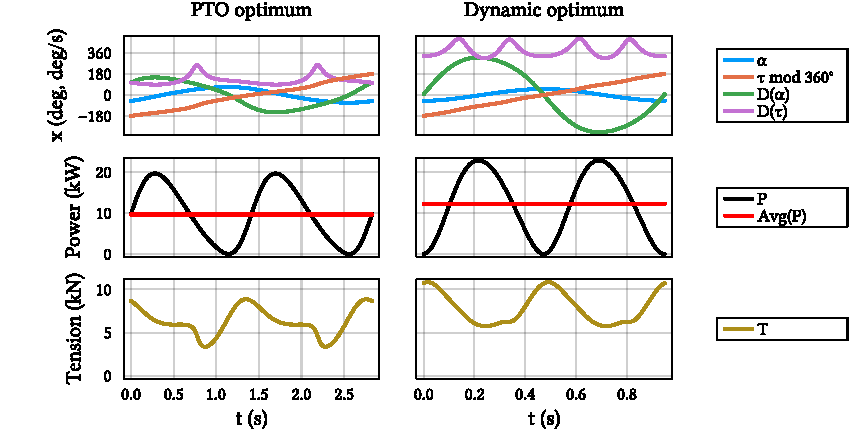
\includegraphics[width=\textwidth]{figs/optimization_timeseries_all.pdf}
    \caption{Time series of the BVP with optimal parameters according to PTO (left) and after dynamic optimization (right).
}
    \label{fig:opt-time-series}
\end{figure}


\begin{figure}[thpb]
    \centering
    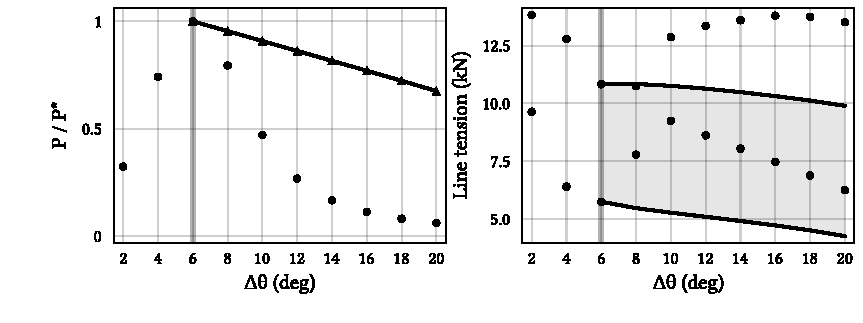
\includegraphics[width=\textwidth]{figs/optimization_dtheta.pdf}
    \caption{Average power, line tension and acceleration \alter{show acceleration?} as $\Delta \theta$ varies.
    The height of the lemniscate has very little impact on the results, therefore we verify our assumption}
    \label{fig:opt-time-series}
\end{figure}

\begin{figure}[thpb]
    \centering
    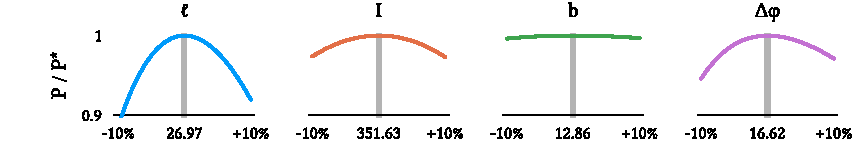
\includegraphics[width=\textwidth]{figs/optimization_landscape.pdf}
    \caption{Average power as the optimization parameters vary.
    The objective landscape is smooth, explaining the easy numerical solving. \alter{which variables are on their bounds ?} \alter{which variables have the most impact?} \alter{could reoptimize other 3 parameters}}
    \label{fig:opt-time-series}
\end{figure}

\begin{figure}[thpb]
  \centering
  \includegraphics{figures/parametrized_optimization_power}
  \caption{Average generated power for optimized (blue) and reference (black) parameters when the reference wind speed $w_0$ is varied.
  The reference curve is generated by fixing the design parameters to the optimal values for a $w_0 = \SI{10}{\meter\per\second}$.}
  \label{fig:parameterized_optimization_power}
\end{figure}

\begin{figure}[thpb]
  \centering
  \includegraphics{figures/parametrized_optimization_tension}
  \caption{Minimum and maximum line tension $\vb F_\ell$ for optimized (blue) and reference (black) parameters.}
  \label{fig:parameterized_optimization_tension}
\end{figure}

\begin{figure}[thpb]
  \centering
  \includegraphics{figures/parametrized_optimization_params}
  \caption{Optimal parameters for each wind speed (color) and and reference parameters fixed at the optimum for $w_0 = \SI{10}{\meter\per\second}$ (black dashed lines).}
  % At this level of operation and despite relatively strong changes in the environmental parameter, the braking coefficient of the arm behaves linearly with respect to wind speed.
  \label{fig:parameterized_optimization_params}
\end{figure}